\documentclass[conference]{IEEEtran}
\IEEEoverridecommandlockouts

\usepackage[T1]{fontenc}
\usepackage[utf8]{inputenc}
\usepackage{textcomp}
\usepackage{cite}
\usepackage{amsmath,amssymb,amsfonts}
\usepackage{graphicx}
\usepackage{booktabs}
\usepackage{tikz}
\usetikzlibrary{arrows.meta,positioning}
\usepackage[hidelinks]{hyperref}

\newcommand{\ERF}{\textsc{ow-erf}}

\begin{document}

\title{Open-World Explained-Rarity Filtering for Health-Insurance Claim Fraud: Problem Formulation, Benchmark Design and Preliminary Synthetic Evidence}

\author{
\IEEEauthorblockN{Ishant Pant}
\IEEEauthorblockA{Lead Author\\
Department of Data Science\\
Manipal University Jaipur\\
Dehmi Kalan, Jaipur, Rajasthan 303007, India\\
ishantpant2332@gmail.com}
\and
\IEEEauthorblockN{Dr. Sandeep Gupta}
\IEEEauthorblockA{Research Supervisor\\
Department of Data Science\\
Manipal University Jaipur\\
Dehmi Kalan, Jaipur, Rajasthan 303007, India}
}

\maketitle

\begin{abstract}
Health-insurance fraud detectors trained on known fraud categories fail in two ways: they force novel schemes into familiar classes (the closed-world assumption), and they treat statistical rarity as evidence of fraud, which penalizes legitimate severe cases such as polytrauma. We formulate \emph{explained-rarity filtering}: a claim should be escalated only if it is both unfamiliar to the model and unexplained by its clinical context. We describe \ERF{}, a pipeline that (i) scores novelty by fusing an energy score and a Mahalanobis distance, (ii) converts the score into a split-conformal $p$-value for approximate control of the false-rejection rate, and (iii) filters rare-but-explained claims with a heteroscedastic expectation model trained on legitimate claims only. We evaluate a tabular prototype on a synthetic claim generator with four fraud mechanisms under leave-one-mechanism-out. In this preliminary setting the conformal stage keeps the benign rejection rate near the nominal $5\%$, and the filter reduces the benign escalation rate to about $0.5\%$, but it also lowers recall on mechanisms whose attributes look clinically plausible. We report this trade-off and the limitations of synthetic-only evaluation. We make no claim about real-world performance.
\end{abstract}

\begin{IEEEkeywords}
health-insurance fraud, open-world recognition, conformal prediction, anomaly detection, graph neural networks
\end{IEEEkeywords}

\section{Introduction}
Large claim volumes in health-insurance systems, including IRDAI-regulated insurance and the AB-PMJAY scheme in India, make exhaustive manual review impractical. Fraud mechanisms such as upcoding, unbundling, phantom billing and collusive referral rings also change over time. Three problems follow.

\begin{enumerate}
\item \textbf{Closed-world classification.} A softmax classifier assigns a new scheme to the nearest known class, often with high confidence.
\item \textbf{Rarity is not fraud.} Pure anomaly scores flag legitimate severe cases because they are rare, complex and expensive.
\item \textbf{Alert fatigue.} Raw scores carry no statistical meaning, so a fixed threshold drifts and review budgets are exceeded.
\end{enumerate}

\textbf{Contributions.} (1) A problem formulation, \emph{explained-rarity filtering}, that separates unfamiliarity from unexplainedness. (2) A pipeline (\ERF{}) combining post-hoc novelty fusion, split-conformal rejection and a heteroscedastic clinical expectation filter. (3) A benchmark protocol with a synthetic claim generator, leave-one-mechanism-out evaluation and leakage control. (4) Preliminary evidence from a tabular prototype, including where the filter hurts.

\section{Related Work}
\textbf{Open-set and open-world recognition.} Open-set recognition~\cite{scheirer2013,geng2021} and out-of-distribution (OOD) baselines~\cite{hendrycks2017,lee2018,liu2020energy} score unfamiliarity from logits or embeddings. On graphs, OpenWGL~\cite{wu2020openwgl} rejects unseen-class nodes with a variational graph autoencoder, and GNNSafe~\cite{wu2023gnnsafe} applies energy-based detection to graph neural networks.

\textbf{Graph fraud and anomaly detection.} CARE-GNN~\cite{dou2020care} counters camouflage with reinforcement-learned neighbor selection, and BWGNN~\cite{tang2022bwgnn} addresses heterophily. DOMINANT~\cite{ding2019dominant} and the PyGOD library~\cite{liu2024pygod} cover reconstruction-based detection, while BOND~\cite{liu2022bond} and GADBench~\cite{tang2023gadbench} provide benchmarks. These methods output novelty or anomaly scores and do not separate rare-but-clinically-explained claims from unexplained ones.

\textbf{Conformal prediction.} Split-conformal methods~\cite{vovk2005,lei2018,angelopoulos2023} give finite-sample marginal guarantees under exchangeability. Barber et al.~\cite{barber2023} study relaxations, and Huang et al.~\cite{huang2023cfgnn} apply conformal prediction to graph neural networks. Temporal claim streams violate exchangeability, so our guarantee is approximate and is tested empirically.

\textbf{Heteroscedastic regression.} Predicting a mean and a variance under a Gaussian likelihood~\cite{nix1994,kendall2017} lets the expected spread grow with severity.

\textbf{Healthcare fraud.} Prior work applies supervised and unsupervised learning to Medicare-style data~\cite{bauder2017}.

\section{Problem Formulation}
Let a claim $v$ have features $x_v$, a graph neighborhood, and a label $y_v$ from benign, known mechanisms, or novel mechanisms. Training sees only benign and known mechanisms. At test time a claim is \emph{unfamiliar} if its conformal $p$-value satisfies $p_v \le \alpha$, and \emph{unexplained} if its clinical inconsistency ratio $a_v$ exceeds a calibrated threshold $\tau$. A claim is escalated if and only if it is both.

To prevent temporal leakage, the embedding of claim $v$ at adjudication time $t$ uses only the causal neighborhood
\begin{equation}
\mathcal{N}_r(v;t)=\{u:(u,v)\in E_r,\; t(u,v)\le t\}.
\end{equation}

\section{Method}
Fig.~\ref{fig:arch} shows the pipeline.

\begin{figure*}[t]
\centering
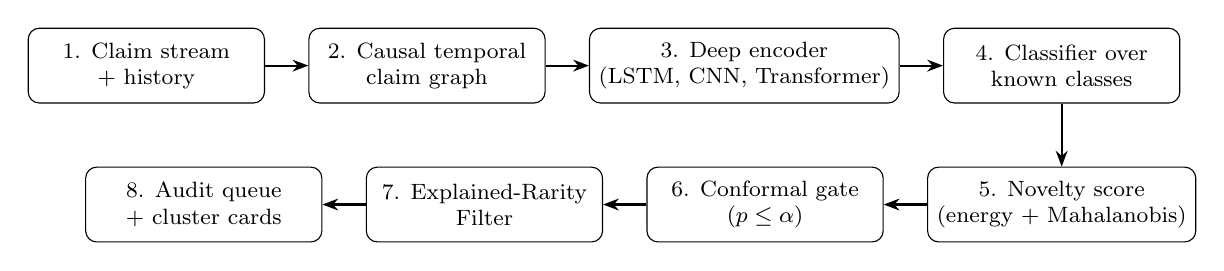
\begin{tikzpicture}[node distance=0.55cm,
  box/.style={draw, rounded corners, align=center, minimum width=3.0cm, minimum height=0.95cm, font=\footnotesize},
  arr/.style={-{Stealth[length=2mm]}, thick}]
\node[box] (a) {1. Claim stream\\+ history};
\node[box, right=of a] (b) {2. Causal temporal\\claim graph};
\node[box, right=of b] (c) {3. Deep encoder\\(LSTM, CNN, Transformer)};
\node[box, right=of c] (d) {4. Classifier over\\known classes};
\node[box, below=0.8cm of d] (e) {5. Novelty score\\(energy + Mahalanobis)};
\node[box, left=of e] (f) {6. Conformal gate\\($p\le\alpha$)};
\node[box, left=of f] (g) {7. Explained-Rarity\\Filter};
\node[box, left=of g] (h) {8. Audit queue\\+ cluster cards};
\draw[arr] (a)--(b); \draw[arr] (b)--(c); \draw[arr] (c)--(d);
\draw[arr] (d)--(e); \draw[arr] (e)--(f); \draw[arr] (f)--(g); \draw[arr] (g)--(h);
\end{tikzpicture}
\caption{Pipeline of \ERF{}. Stages 1--4 learn representations; stages 5--8 make the decision.}
\label{fig:arch}
\end{figure*}

\subsection{Encoder}
The full system builds a time-stamped heterogeneous graph (claim, beneficiary, hospital, doctor, package, diagnosis) and encodes it with R-GCN~\cite{schlichtkrull2018} or HGT~\cite{hu2020hgt} using PyTorch Geometric~\cite{fey2019pyg}. We also describe three complementary branches whose individual value must be established by ablation: an LSTM over the provider's recent claim history, a one-dimensional CNN over the ordered procedure-code sequence of a claim, and a Transformer encoder over relational-context tokens. \emph{The preliminary results below use a tabular encoder only; the deep branches are implemented but not yet trained or evaluated.}

\subsection{Novelty score}
From classifier logits $z$, the energy is
\begin{equation}
E(x)=-T\log\sum_{k}\exp(z_k/T).
\end{equation}
The Mahalanobis score $M(h)$ is the minimum over known classes of the squared Mahalanobis distance of embedding $h$ to the class mean under the class covariance. With $F_E$ and $F_M$ the empirical CDFs of $E$ and $M$ on training data, the fused score is
\begin{equation}
u=\tfrac12 F_E(E)+\tfrac12 F_M(M).
\end{equation}

\subsection{Conformal rejection}
On a calibration set disjoint from training and containing only known-class claims, with $n$ calibration scores $u_i$, the $p$-value is
\begin{equation}
p_v=\frac{1+\#\{i:u_i\ge u_v\}}{n+1},
\end{equation}
and a claim is rejected as unfamiliar when $p_v\le\alpha$ with $\alpha=0.05$.

\subsection{Explained-Rarity Filter}
A heteroscedastic model trained on benign claims only predicts a mean $\mu_j$ and standard deviation $\sigma_j$ for $j\in\{\text{log-amount},\text{length of stay}\}$ from \emph{exogenous} inputs (a severity proxy from prior history, comorbidity count, age) by minimizing
\begin{equation}
\mathcal{L}_g=\frac{1}{N}\sum_{i}\sum_{j}\Big[\ln\sigma_{ij}+\frac{(o_{ij}-\mu_{ij})^2}{2\sigma_{ij}^2}\Big].
\end{equation}
The inconsistency ratio is
\begin{equation}
a_v=\max_j\max\Big\{0,\frac{o_j-\mu_j}{\sigma_j}\Big\}.
\end{equation}
The threshold $\tau$ is set as a quantile of $a_v$ on benign calibration claims rather than by hand. The expectation model must not condition on fields a fraudster controls, such as the claimed diagnosis code; otherwise upcoding would make fraud look explained.

\subsection{Planned components}
Episodic pseudo-novel training masks one known fraud class per episode and adds a squared-hinge energy-margin loss to cross-entropy. HDBSCAN~\cite{campello2013} groups escalated claims into typologies. Neither is evaluated here.

\section{Experimental Protocol}
\textbf{Data.} A synthetic generator produces benign claims, $5\%$ rare-severe legitimate claims, and four mechanisms: upcoding, unbundling, phantom billing, and collusion (represented in the prototype by two proxy features only). The fraud rate is $10\%$.

\textbf{Splits and metrics.} Leave-one-mechanism-out: train and calibrate on benign plus three known mechanisms, test on all four. We use five random seeds and $9{,}000$ test claims per run. Metrics are recall on the held-out mechanism, the benign rejection rate, and the fraction of rare-severe legitimate claims flagged, each before and after the filter.

\textbf{Baseline.} Isolation Forest~\cite{liu2008iforest}, with its alert count matched to the number of \ERF{} escalations.

\section{Preliminary Results}
Table~\ref{tab:res} reports means over five seeds from the released script. The conformal stage rejects between $4.3\%$ and $4.6\%$ of benign claims, close to the nominal $5\%$ on this i.i.d.\ synthetic split; this does not demonstrate validity under temporal drift. After the filter, benign escalation falls to about $0.5\%$. The filter cuts flags on rare-severe legitimate claims most clearly for phantom billing ($13.3\%\to2.6\%$). It also lowers recall: for collusion the drop is large ($0.586\to0.211$), because those claims look clinically plausible and would require graph structure that this prototype lacks. At a matched alert count, Isolation Forest recalls only $0.02$--$0.04$ of the three attribute-level mechanisms ($0.20$ for collusion) while flagging $22\%$--$28\%$ of rare-severe legitimate claims. All of these results are conditional on the generator.

\begin{table}[t]
\caption{Leave-one-mechanism-out results (synthetic data, tabular prototype, mean of 5 seeds). Recall is on the held-out mechanism; ``Rare flag'' is the fraction of rare-severe legitimate claims flagged.}
\label{tab:res}
\centering
\small
\begin{tabular}{lcccc}
\toprule
Held-out & Recall & Recall & Rare flag & Rare flag\\
mechanism & conf. & +ERF & conf. & +ERF\\
\midrule
Upcoding & 0.574 & 0.560 & 0.026 & 0.006\\
Unbundling & 0.493 & 0.372 & 0.020 & 0.003\\
Phantom billing & 0.496 & 0.411 & 0.133 & 0.026\\
Collusion (proxy) & 0.586 & 0.211 & 0.016 & 0.002\\
\bottomrule
\end{tabular}
\end{table}

\section{Limitations}
The evidence is synthetic only, and the generator encodes our assumptions about severity and cost. The prototype has no graph encoder, so collusion is only approximated by two tabular features. Novelty scoring is post-hoc, without episodic pseudo-novel training. The conformal guarantee is marginal and assumes exchangeability, which temporal streams violate, and it does not cover the filter stage. If the filter's severity inputs can be manipulated, fraud can be explained away. Only one baseline has been run so far. Finally, wrongly escalated claims delay care, so any deployment requires human review and an audit of group-wise error rates.

\section{Conclusion and Future Work}
Explained-rarity filtering trades recall for far fewer false alarms on legitimate rare claims. Next steps are the graph encoder, trained and ablated deep branches, the full baseline set, temporal conformal tests, and evaluation on a real public claims dataset.

\section*{Data and Code Availability}
No patient data are used. Code and generator: \texttt{https://github.com/USERNAME/REPO} (to be added with an archived DOI and the exact commit used for Table~\ref{tab:res}).

\section*{Acknowledgment}
The authors used Claude (Anthropic) to assist in drafting the manuscript text, the experiment code and the presentation slides. The authors reviewed and edited the content and take full responsibility for it.

\bibliographystyle{IEEEtran}
\bibliography{references}

\end{document}
